\documentclass[UTF8]{ctexart}
\usepackage{graphicx}
\usepackage{subfigure}
\usepackage{amsmath}
\usepackage{geometry}
\usepackage{enumerate}
\usepackage{cite}
\usepackage{booktabs}
\usepackage{listings}
\usepackage{titletoc}

\lstset{language=C++}
\lstset{breaklines}%这条命令可以让LaTeX自动将长的代码行换行排版
\lstset{extendedchars=false}%这一条命令可以解决代码跨页时,章节标题,页眉等汉字不显示的问题

\geometry{left=2cm,right=2cm,top=2cm,bottom=2cm}

\title{\heiti 《流体力学高精度数值解法》 \\ 大作业}
\author{SX1501021 仓宇}
\date{\today}

\bibliographystyle{plain}

\begin{document}
\maketitle
\setcounter{page}{0}
\thispagestyle{empty}
\clearpage

\tableofcontents
\clearpage

\section{问题描述}
使用基于Taylor级数展开与最小二乘法的格子玻尔兹曼方法(TLLBM,Taylor series expansion and Least square based Lattice Boltzmann Method)来模拟二维圆柱绕流问题。要求如下:
\begin{itemize}
\item 分别考察雷诺数$Re=20,40,100,400$时的流场;
\item 比较不同精细程度的网格对数值解的影响;
\item 给出速度残差或密度残差随时间的变化;
\item 给出升力系数$C_L$与阻力系数$C_D$随时间的变化;
\item 给出流线图和涡量等值线图。
\end{itemize}

\section{TLLBM方法概述}
本文以D2Q9模型为例,特殊声明除外。
\subsection{LBM概述}
\indent 在LBM中,任一节点在给定方向上的的密度平衡分布$f_i$由两部分组成:平衡部分与非平衡部分,即:
\begin{equation}
f_i=f_i^{(eq)}+f_i^{(neq)} 
\end{equation}
\indent 每个节点上的物理量(如$\rho,u,v$)由该节点上各个方向的密度分布$f_i$共同决定,即:
\begin{equation}
 \rho= \sum_{i=0}^{Q-1}f_i 
\end{equation}
\begin{equation} 
u= \frac{1}{\rho}\sum_{i=0}^{Q-1}{f_i cx_i} 
\end{equation}
\begin{equation} 
v= \frac{1}{\rho}\sum_{i=0}^{Q-1}{f_i cy_i}
\end{equation}
\indent 上式中$cx_i,cy_i$由具体模型给定。\\
\indent 反过来,每点上的物理量又决定了该点上各个方向密度分布中的平衡部分,即:
\begin{equation} 
f_i^{(eq)} = F(\rho,u,v)
\end{equation}
\indent 上式中的F由所采用的计算模型决定。\\
\indent 因此,节点上各个方向的密度分布$f_i$与节点上的物理量(如$\rho,u,v$)形成一种等价关系。\\
\indent 从上面公式可以看出一些有趣的想法:LBM认为在任意一点上的密度并不沿着周向连续均匀分布,相反,它认为密度的分布是间断的,是按照一定的比例集中地分布在若干个给定的方向上。进一步,对于速度分量来说,各个方向上的密度分布$f_i$起到类似权重的效果。\\
\indent LBM的想法基于Boltzmann方程,也就是每点在下一时间步的密度分布$f_i(t+dt)$由当前不稳定的那部分$f_i^{(neq)}(t)$引起的碰撞和对流导致。碰撞的具体形式是每个LBM模型的核心所在。碰撞后粒子还要做对流运动,从而迁移到下一个位置,在LBGK中,描述粒子碰撞与迁移的函数如下:
\begin{equation} 
 f_i(P^\prime,t+dt)=f_i(P,t)-\frac{1}{\tau}[f_i(P,t)-f_i^{(eq)}(P,t)] 
\end{equation}
\indent 这样,我们便建立了对LBM的基本认识。

\subsection{理解TLLBM}
简单地说,TLLBM是一种基于LBM的时间推进方法,在给定初始条件和边界条件后逐次推进时间步,从而模拟了全流场的演变。TLLBM不同于传统方法的地方在于它为了得到网格点在下一时间步上的状态量而使用的方法。\\
\indent 在TLLBM中,已知t时刻的所有节点的密度分布,为了求P点在$t+dt$时刻的密度分布,TLLBM首先用标准的LBM方法求得周围9个点在$t+dt$时刻的密度分布,然后再用这9个点在$t+dt$时刻的密度分布来近似估计P点在$t+dt$时刻的密度分布,从而完成了时间步的推进。\\
\indent 需要注意的是标准的LBM方法求得的在$t+dt$时刻的密度分布是\emph{迁移后}的节点在新的位置上的分布,而不是原始点在t+dt时刻的密度分布,这也是引入Taylor级数展开和最小二乘法的原因。下面将详细阐释TLLBM做近似估计的原理。\\
\indent 首先,通过标准的LBM得到P点周围9点碰撞迁移后的密度分布,如下所示:
\begin{figure}[htbp]
\centering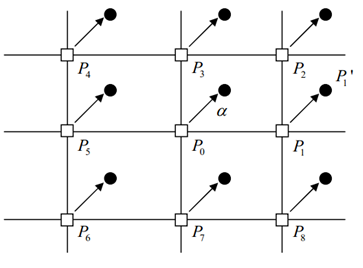
\includegraphics[width=5.5cm,height=4.5cm]{../pic/9pts.png}
\caption{粒子迁移示意图}
\end{figure}\\
\indent 注意这一步的操作包含了节点的所有方向,图中只是沿着一个方向的迁移示意。\\
\indent 记第k个节点沿i方向经过碰撞、迁移得到的中间点在t+dt时刻的密度为$g_{i:k}$,则有:
\begin{equation} 
g_{i:k}= f_i(P_k^\prime,t+dt)=f_i(P_k,t)-\frac{1}{\tau}[f_i(P_k,t)-f_i^{(eq)}(P_k,t)] \ \ \  k=0...8
\end{equation}
\indent 为了求$f_i(P,t+dt)$,我们想办法用这9个点来估计P点在t+dt时刻的密度分布。将上述9点在P点做Taylor展开,保留到二阶,得到的结果如下:
\begin{equation}
\begin{split}
&f_i(P_k^\prime,t+dt)=f_i(P,t+dt)+\Delta x_{P_k} \frac{\partial f_i(P,t+dt)}{\partial x} +\Delta y_{P_k} \frac{\partial f_i(P,t+dt)}{\partial y}\\
&\qquad \qquad \qquad + \frac{1}{2} {\Delta x_{P_k}}^2 \frac{\partial^{2} f_i(P,t+dt)}{\partial x^{2}}+\frac{1}{2} {\Delta y_{P_k}}^2 \frac{\partial^{2} f_i(P,t+dt)}{\partial y^{2}} \\
&\qquad \qquad \qquad + \Delta x_{P_k} \Delta y_{P_k} \frac{\partial^{2} f_i(P,t+dt)}{{\partial x} {\partial y}}
\end{split}
\end{equation}
\indent 其中$\Delta x_{P_k}=x_{P_k}+cx_i dt - x_P$,$\Delta y_{P_k}=y_{P_k}+cy_i dt - y_P$,即中间点$P_k^\prime$与P点的距离。\\
\indent 对于每一个点的泰勒展开,上式中$f_i(P,t+dt), \frac{\partial f_i(P,t+dt)}{\partial x}, \frac{\partial f_i(P,t+dt)}{\partial y}, \frac{\partial^{2} f_i(P,t+dt)}{\partial x^{2}}, \frac{\partial^{2} f_i(P,t+dt)}{\partial y^{2}}, \frac{\partial^{2} f_i(P,t+dt)}{{\partial x} {\partial y}}$这6个量均为未知量,而$\Delta x_{P_k}, \Delta y_{P_k}$均是已知的,因此我们有9个方程,6个未知量。写成矩阵的形式如下:
\begin{equation}
{\begin{pmatrix}
1 & \Delta x_{P_0} & \Delta y_{P_0} & \frac{1}{2} {\Delta x_{P_0}}^2 & \frac{1}{2} {\Delta y_{P_0}}^2 & \Delta x_{P_0} \Delta y_{P_0} \\
1 & \Delta x_{P_1} & \Delta y_{P_1} & \frac{1}{2} {\Delta x_{P_1}}^2 & \frac{1}{2} {\Delta y_{P_1}}^2 & \Delta x_{P_1} \Delta y_{P_1} \\
1 & \Delta x_{P_2} & \Delta y_{P_2} & \frac{1}{2} {\Delta x_{P_2}}^2 & \frac{1}{2} {\Delta y_{P_2}}^2 & \Delta x_{P_2} \Delta y_{P_2} \\
1 & \Delta x_{P_3} & \Delta y_{P_3} & \frac{1}{2} {\Delta x_{P_3}}^2 & \frac{1}{2} {\Delta y_{P_3}}^2 & \Delta x_{P_3} \Delta y_{P_3} \\
1 & \Delta x_{P_4} & \Delta y_{P_4} & \frac{1}{2} {\Delta x_{P_4}}^2 & \frac{1}{2} {\Delta y_{P_4}}^2 & \Delta x_{P_4} \Delta y_{P_4} \\
1 & \Delta x_{P_5} & \Delta y_{P_5} & \frac{1}{2} {\Delta x_{P_5}}^2 & \frac{1}{2} {\Delta y_{P_5}}^2 & \Delta x_{P_5} \Delta y_{P_5} \\
1 & \Delta x_{P_6} & \Delta y_{P_6} & \frac{1}{2} {\Delta x_{P_6}}^2 & \frac{1}{2} {\Delta y_{P_6}}^2 & \Delta x_{P_6} \Delta y_{P_6} \\
1 & \Delta x_{P_7} & \Delta y_{P_7} & \frac{1}{2} {\Delta x_{P_7}}^2 & \frac{1}{2} {\Delta y_{P_7}}^2 & \Delta x_{P_7} \Delta y_{P_7} \\
1 & \Delta x_{P_8} & \Delta y_{P_8} & \frac{1}{2} {\Delta x_{P_8}}^2 & \frac{1}{2} {\Delta y_{P_8}}^2 & \Delta x_{P_8} \Delta y_{P_8}
\end{pmatrix}}
{\begin{pmatrix}
f_i(P,t+dt) \\
\frac{\partial f_i(P,t+dt)}{\partial x} \\
\frac{\partial f_i(P,t+dt)}{\partial y} \\
\frac{\partial^{2} f_i(P,t+dt)}{\partial x^{2}} \\
\frac{\partial^{2} f_i(P,t+dt)}{\partial y^{2}} \\
\frac{\partial^{2} f_i(P,t+dt)}{{\partial x} {\partial y}}
\end{pmatrix}}
={\begin{pmatrix}
f_i(P_0^\prime,t+dt) \\
f_i(P_1^\prime,t+dt) \\
f_i(P_2^\prime,t+dt) \\ 
f_i(P_3^\prime,t+dt) \\ 
f_i(P_4^\prime,t+dt) \\ 
f_i(P_5^\prime,t+dt) \\
f_i(P_6^\prime,t+dt) \\
f_i(P_7^\prime,t+dt) \\
f_i(P_8^\prime,t+dt)
\end{pmatrix}}
\end{equation}
\indent 将这3个矩阵从左到右依次记为$[S_i],\{V_i\},\{g_i\}$。显然这个矩阵方程无解,为了求得近似解,我们采用最小二乘的方法求得$\{V_i\}$的近似解,结果如下:
\begin{equation}
\{V_i\}=({[S_i]}^ \mathrm{T} {[S_i]})^{-1} {[S_i]}^ \mathrm{T} \{g_i\} = [A_i] \{g_i\}
\end{equation}
\indent 至此,我们便求得i方向上P点在t+dt时刻的密度$f_i(P,t+dt)$,其它方向以此类推即可。\\
\indent 需要注意的是由于P点0方向速度为0,所以P点在0方向上没有迁移,因此P点在0方向上$t+dt$时刻的密度可由标准LBM直接得到,无需做Taylor展开来近似估算。

\clearpage

\section{问题分析}
\subsection{网格选取}
求解的一个关键在于网格,虽然上述分析中并未详细说明所采用的是结构网格还是非结构网格,但实际上LBM采用的网格就是真实物理空间上的网格,并不存在从计算域到真实物理空间的转换。结构网格与非结构网格均适用。本文采用贴体非结构网格,如下所示:
\begin{figure}[htbp]\centering
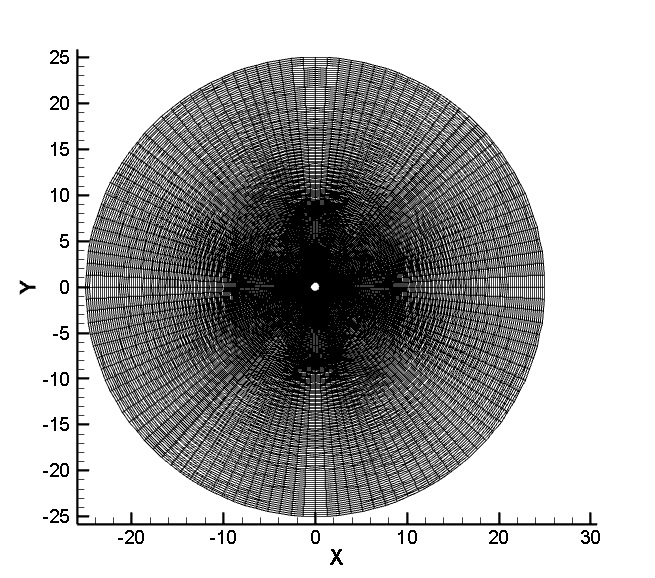
\includegraphics[width=5cm]{../pic/mesh.jpg}
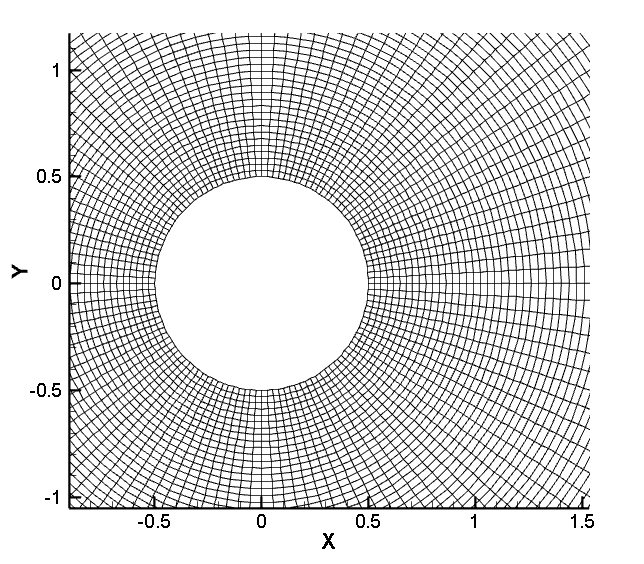
\includegraphics[width=5cm]{../pic/mesh_local.PNG}
\caption{圆柱贴体网格}
\end{figure}

\subsection{初始条件与边界条件}
\indent 求解的另一关键点在于初始条件与边界条件。对于远场,我们认为最外层网格上的物理量不随时间变化,因此在迭代的过程中并不计算或更新最外层的网格,而是始终保持其上的物理量不变。\\
\indent 对于物面,由于存在粘性,物面上的速度必然为始终0,这需要我们在迭代的过程中始终保持速度为0不变。物面除的密度是可变的,反应了压强的变化,因此不作手工修正。\\
\indent 由于我们对每个点的计算采用了其周围9个点的信息,对于物面上的点来说并不存在这样的9点,因此,我们还要再物面内部虚拟放置一层网格,记这层虚拟的网格的层号为0,物面网格的层号为1,这层虚拟的网格是由第2层网格关于物面镜像得到,也就是说我们用第2层网格上的密度分布来代替第0层上的密度分布,从而使得物面上的计算可以归一化处理。因此在每次迭代初始,要用第2层网格的信息来更新第0层网格的信息。\\
\indent 初始时,设包括虚拟层0在内共有N层网格,为了便于计算设1--N-1层网格上的密度均为1,设2--N-1层网格上的速度均为水平向右,且大小相同,具体大小由测试马赫数Ma给定。\\
\indent 设定好初始条件与边界条件后便可开始迭代计算。迭代过程中需要注意的是要遍历所有方向,并且需要注意的是要将流场中全部节点在t+dt时刻的密度分布都求出来后才可以用$f(t+dt)$来代替$f(t)$,不能一边计算,一边迭代。

\subsection{迭代}
首先,物面的网格比较特殊,需要镜像虚拟一层网格才能使用TLLBM。\\
其次,对每点的迭代需要依次更新该点的\emph{所有方向}上的密度,不要漏掉或搞错次序。0方向在这里又是一个比较特殊的情况,由于该方向的速度为0,不会发生迁移,因此做LBM后得到的结果就是该点在t+dt时刻在该方向上的密度。而剩下的1--8方向则需要先对周围9点先做LBM,然后在按前述方法进行插值估计,从而得到该点在t+dt时刻在该方向上的密度。

\clearpage

\section{编程实现}
\subsection{优化加速}
为了加速计算,可以采用\emph{空间换时间}的策略:由于在整个迭代过程中每个点的xy坐标不变,节点迁移的速度是给定的,迁移的时间步长也是不变的,因此可以预先将每个网格节点在1--8方向上的矩阵$\{S_i\}$都求出来,进而可以求出矩阵$[A_i]$,由于计算$f_i(P,t+dt)$只用到了矩阵$[A_i]$的第一行,所以记下每个节点1--8方向上的A矩阵的第一行的9个元素即可。\\
\indent 进一步地,还可以预先存下每个点周围8个点的序号,以便加速存取数据,由于本算例的网格点最多不超过$10^5$,这一优化相对来说性价比不高,因此本文并未做次优化,但是若在工程中使用该方法,这一优化是值得的。\\
\indent 矩阵求逆等运算可以直接用外部库,本算例用的是基于C++的Eigen3,接口灵活方便且实现的效率高!预处理过程中对于每一点在每个方向上的矩阵$[A_i]$,只需如下一行语句即可:
\begin{lstlisting}
auto curA = ((S.transpose()*S).inverse()*S.transpose()).eval();
\end{lstlisting}

\subsection{程序流程}
结合上一节的讨论,程序的流程如下:
\begin{figure}[htbp]\centering
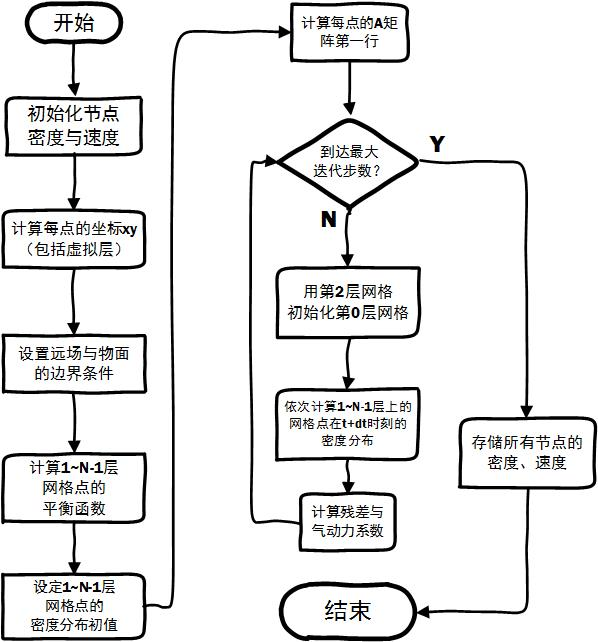
\includegraphics[height=12cm,width=11cm]{../pic/flowchart.jpg}
\caption{程序流程图}
\end{figure}
\clearpage

\section{结果分析}
给出Re=20,40,100,200时的流线图、涡量云图、残差收敛曲线、气动力系数。并进一步探究网格精细程度对数值结果的影响。
\subsection{Re=20}
从下面4幅图可见在Re=20时,圆柱背风区产生两个较小的涡,但并未脱离,流场上下对称,速度残差与密度残差均随时间步的推进而逐渐减小,最终取余平缓,升力系数保持为0。
\begin{figure}[htbp]\centering
\begin{minipage}{7cm}
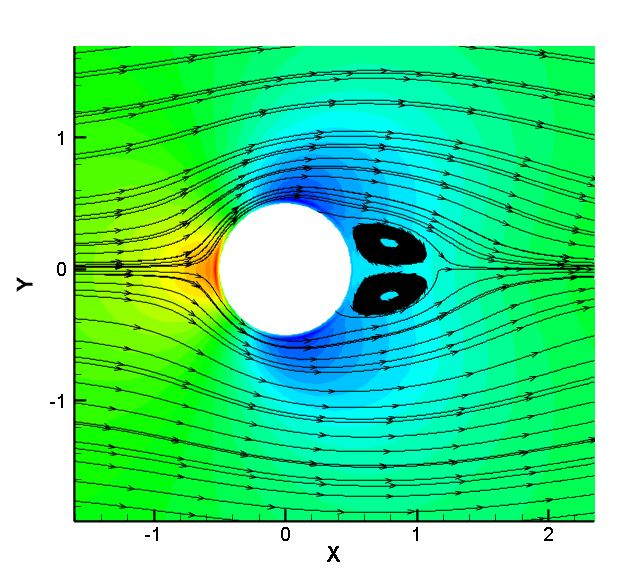
\includegraphics[height=7cm,width=7cm]{../pic/Streamline_20.JPG}
\caption{Re=20 \ 流线图}
\end{minipage}
\begin{minipage}{7cm}
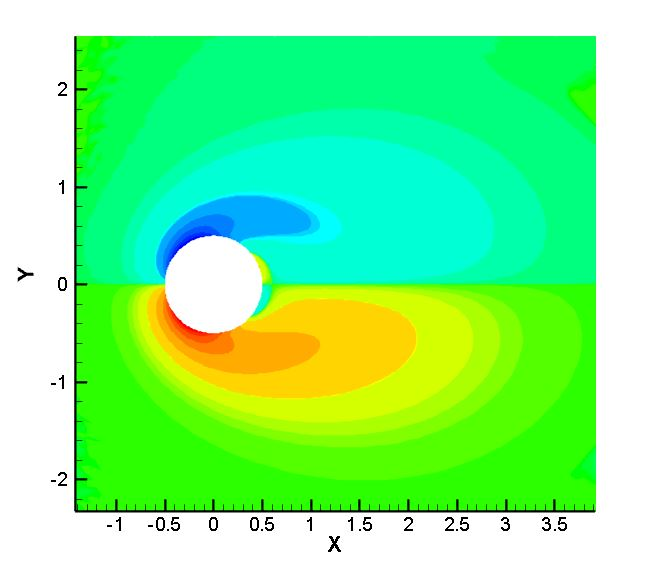
\includegraphics[height=7cm,width=7cm]{../pic/Vorticity_20.JPG}
\caption{Re=20 \ 涡量云图}
\end{minipage}

\begin{minipage}{7cm}
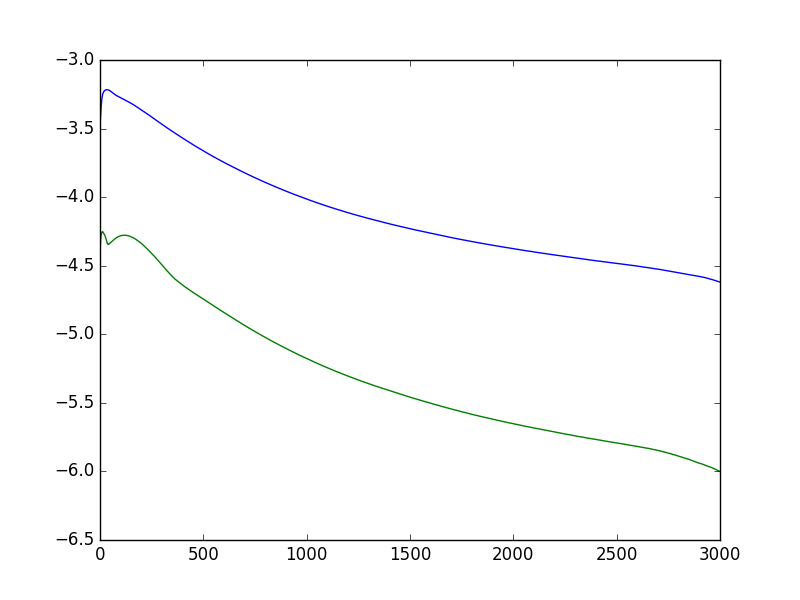
\includegraphics[height=7cm,width=7cm]{../pic/Residue_20.png}
\caption{Re=20 \ 残差图}
\end{minipage}
\begin{minipage}{7cm}
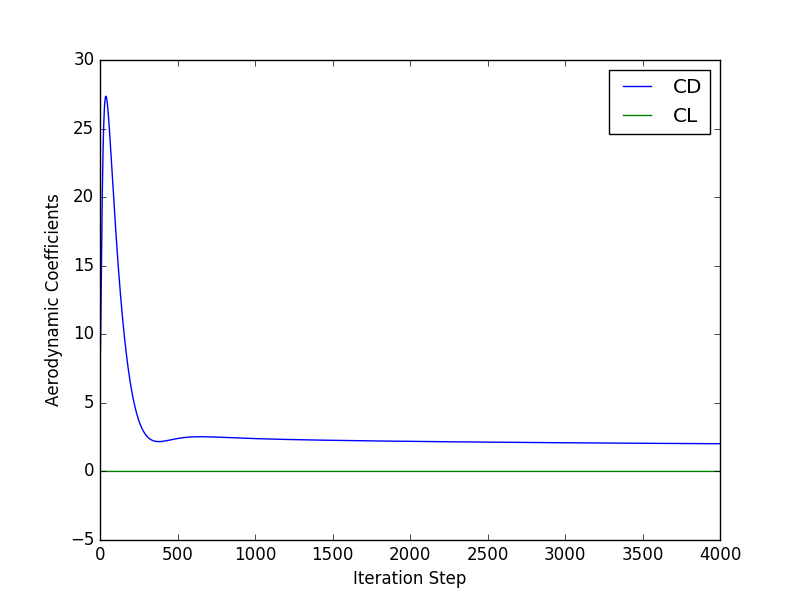
\includegraphics[height=7cm,width=7cm]{../pic/Aerodynamics_20.png}
\caption{Re=20 \ 气动力系数}
\end{minipage}
\end{figure}
\clearpage

\subsection{Re=40}
从下面4幅图可见在Re=40时,圆柱背风区产生两个涡,虽然尚未脱离,但从涡量云图上可以看出随着Re的增大,圆柱后面的涡被拉长了,流场上下对称,速度残差与密度残差均随时间步的推进而逐渐减小,最终取余平缓,升力系数保持为0。
\begin{figure}[htbp]\centering
\begin{minipage}{7cm}
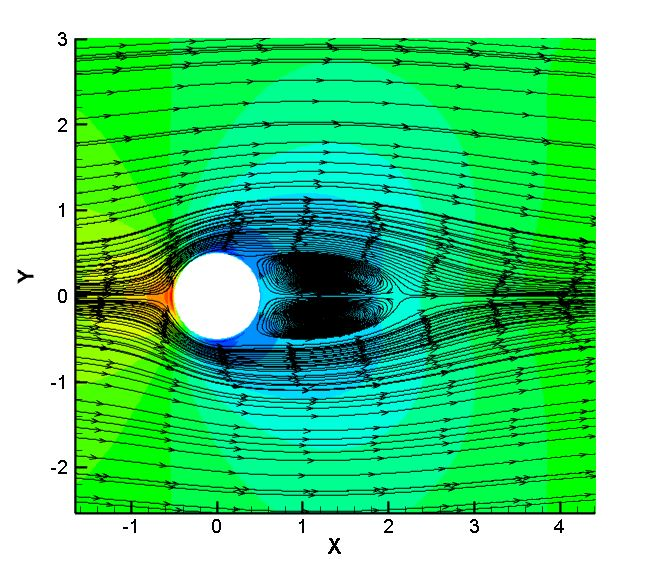
\includegraphics[height=7cm,width=7cm]{../pic/Streamline_40.JPG}
\caption{Re=40 \ 流线图}
\end{minipage}
\begin{minipage}{7cm}
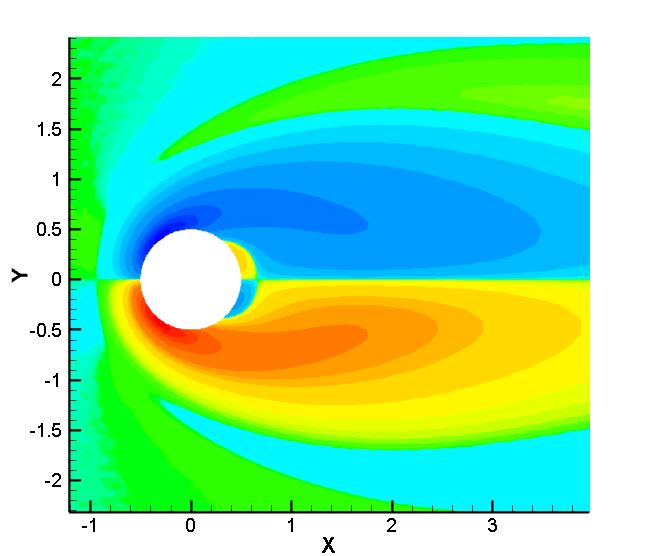
\includegraphics[height=7cm,width=7cm]{../pic/Vorticity_40.JPG}
\caption{Re=40 \ 涡量云图}
\end{minipage}

\begin{minipage}{7cm}
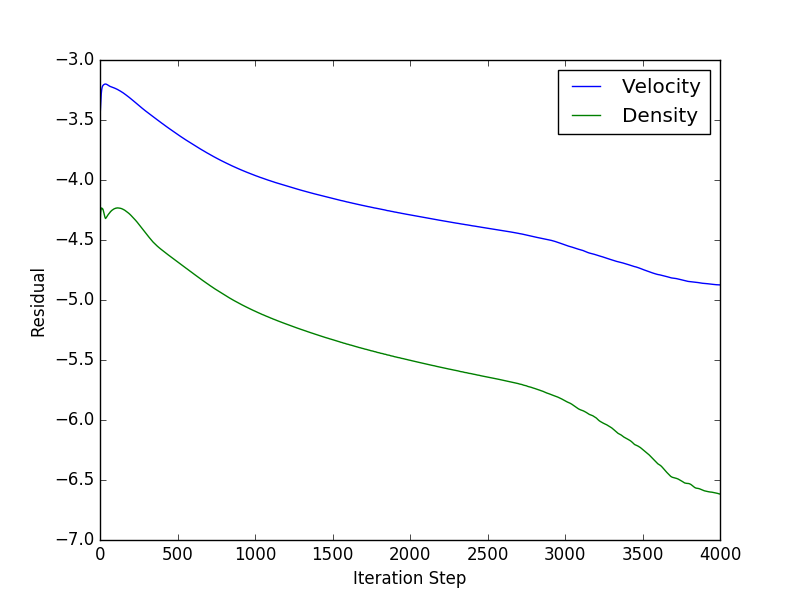
\includegraphics[height=7cm,width=7cm]{../pic/Residue_40.png}
\caption{Re=40 \ 残差图}
\end{minipage}
\begin{minipage}{7cm}
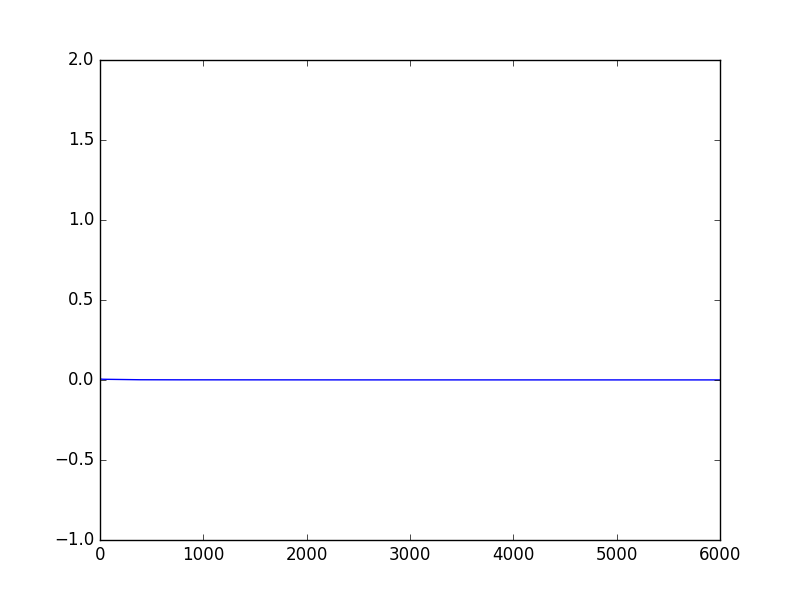
\includegraphics[height=7cm,width=7cm]{../pic/Aerodynamics_40.png}
\caption{Re=40 \ 气动力系数}
\end{minipage}
\end{figure}
\clearpage

\subsection{Re=100}
从下面4幅图可见在Re=100时,圆柱背风区的两个涡被进一步拉长,流场上下对称,速度残差与密度残差均随时间步的推进而逐渐减小,虽然略有抖动,但最终趋于平缓,升力系数保持为0。
\begin{figure}[htbp]\centering
\begin{minipage}{7cm}
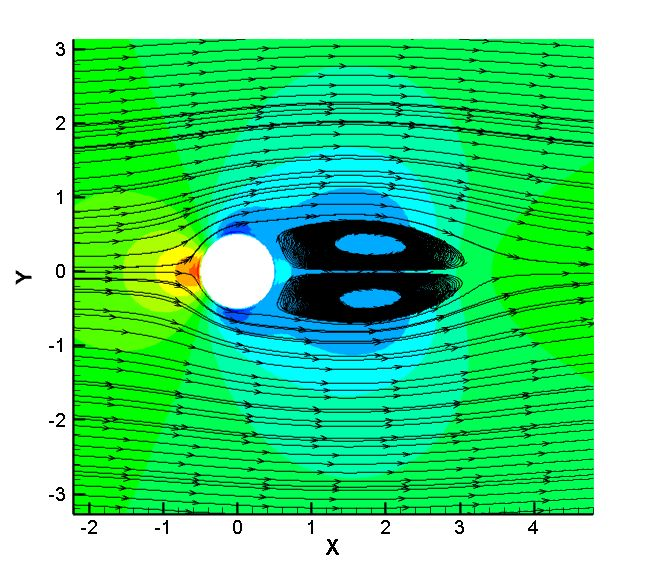
\includegraphics[height=7cm,width=7cm]{../pic/Streamline_100.JPG}
\caption{Re=100 \ 流线图}
\end{minipage}
\begin{minipage}{7cm}
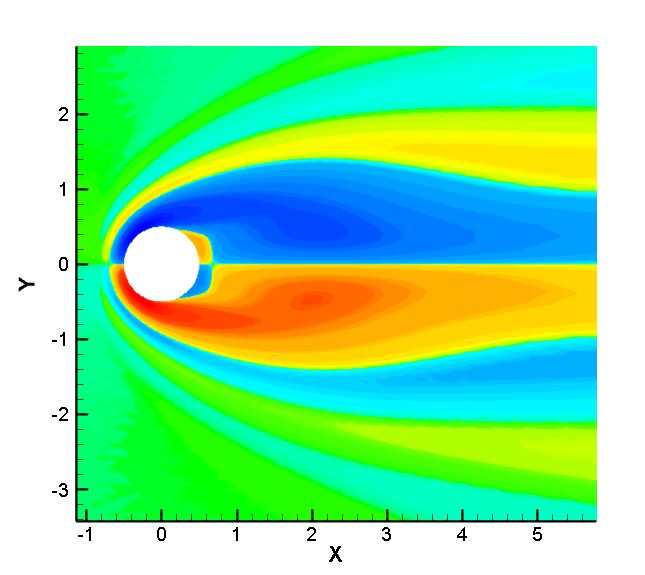
\includegraphics[height=7cm,width=7cm]{../pic/Vorticity_100.JPG}
\caption{Re=100 \ 涡量云图}
\end{minipage}

\begin{minipage}{7cm}
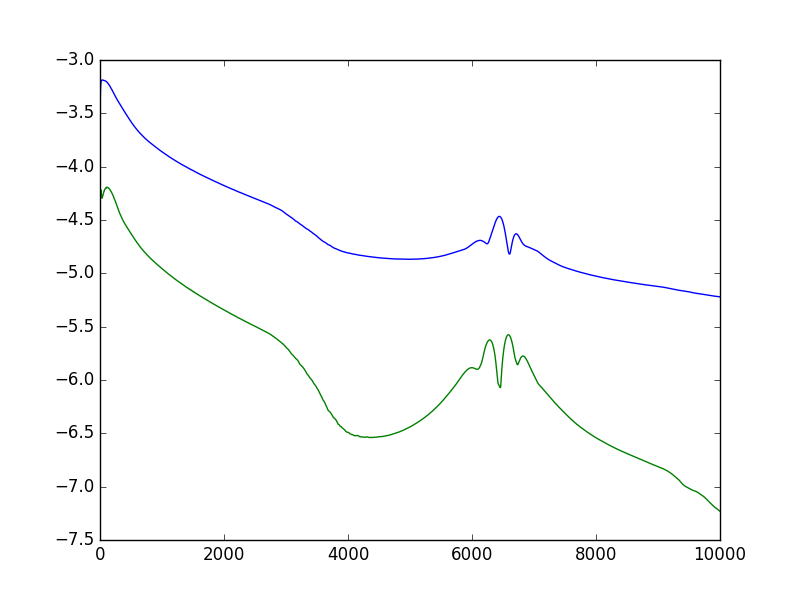
\includegraphics[height=7cm,width=7cm]{../pic/Residue_100.png}
\caption{Re=100 \ 残差图}
\end{minipage}
\begin{minipage}{7cm}
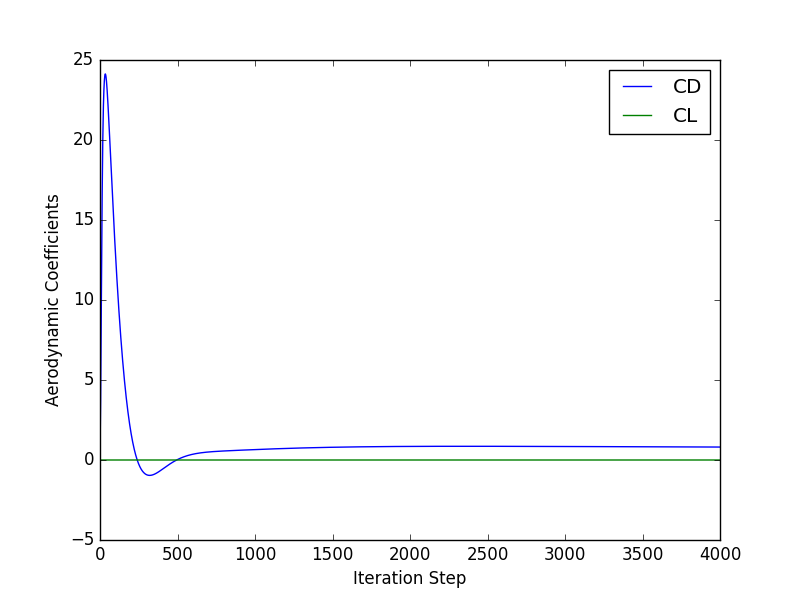
\includegraphics[height=7cm,width=7cm]{../pic/Aerodynamics_100.png}
\caption{Re=100 \ 气动力系数}
\end{minipage}
\end{figure}
\clearpage

\subsection{Re=200}
从下面4幅图可见在Re=200时,圆柱背风区的两个大涡已经脱落,并在背风区又产生了两个小的涡,流场上下对称,速度残差与密度残差均随时间步的推进而逐渐减小,最终取余平缓,升力系数保持为0。
\begin{figure}[htbp]\centering
\begin{minipage}{7cm}
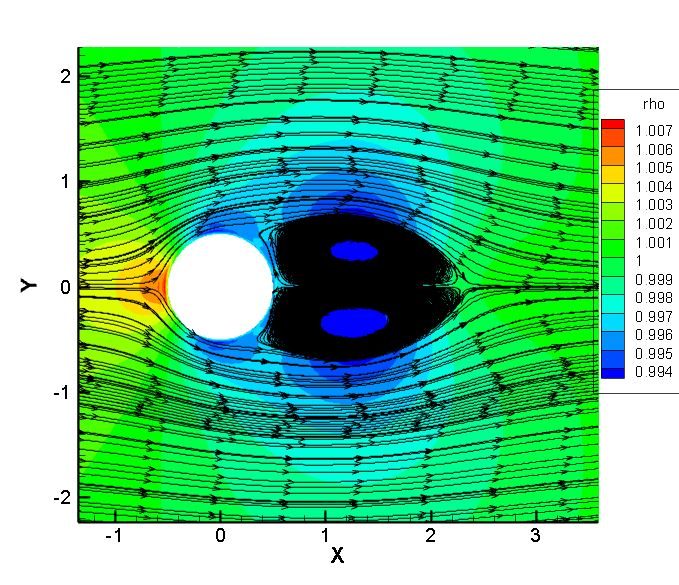
\includegraphics[height=7cm,width=7cm]{../pic/Streamline_200.JPG}
\caption{Re=200 \ 流线图}
\end{minipage}
\begin{minipage}{7cm}
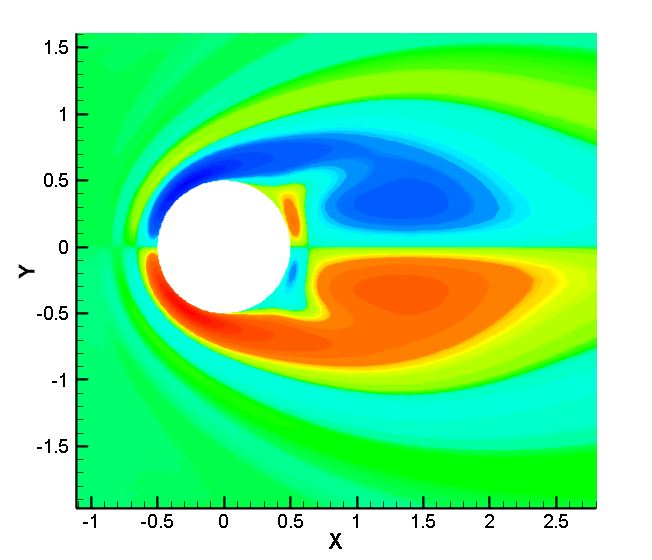
\includegraphics[height=7cm,width=7cm]{../pic/Vorticity_200.JPG}
\caption{Re=200 \ 涡量云图}
\end{minipage}

\begin{minipage}{7cm}
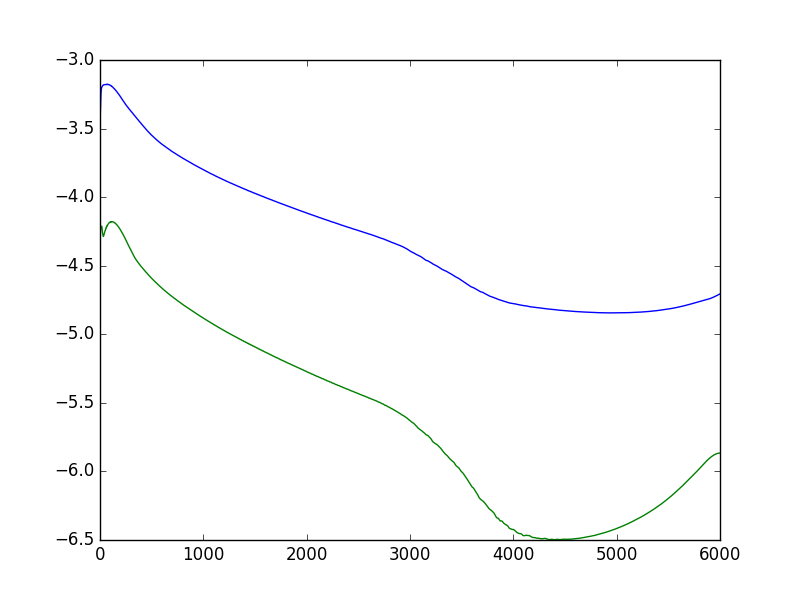
\includegraphics[height=7cm,width=7cm]{../pic/Residue_200.png}
\caption{Re=200 \ 残差图}
\end{minipage}
\begin{minipage}{7cm}
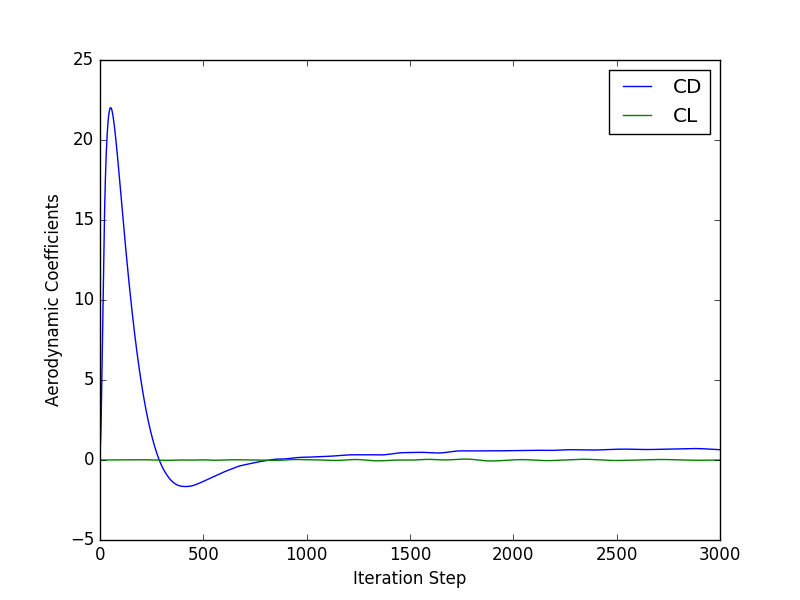
\includegraphics[height=7cm,width=7cm]{../pic/Aerodynamics_200.png}
\caption{Re=200 \ 气动力系数}
\end{minipage}
\end{figure}
\clearpage

\subsection{网格对数值结果的影响}
上述结果采用的网格均相同,设远场距离为50倍的半径长,从物面到远场使用了240层网格,每层网格上有180个节点均匀分布,径向的240层网格并非均匀分布,以1.2为系数做了拉伸变换。作为对比,我们考察在Re=200时,将径向网格数量减少50\%,周向网格密度保持不变的情况下的数值结果,流场、涡量、残差、气动力系数如下:
\begin{figure}[htbp]\centering
\begin{minipage}{7cm}
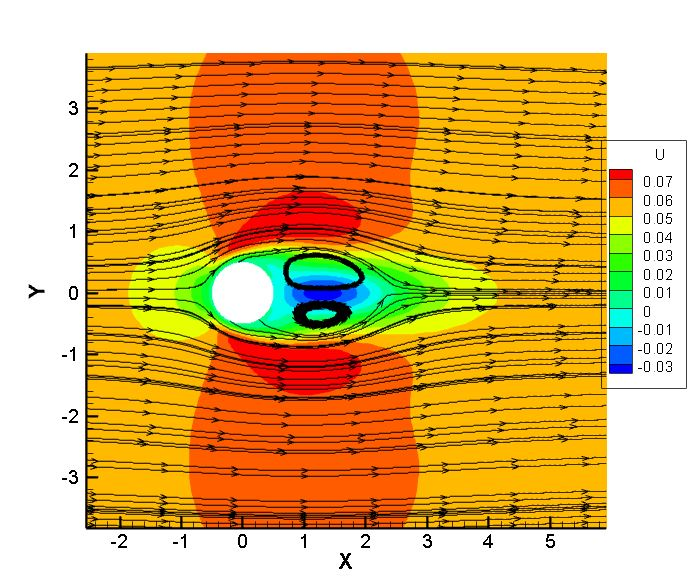
\includegraphics[height=7cm,width=7cm]{../pic/Streamline_Contrast.JPG}
\caption{Re=200 \ 流线图}
\end{minipage}
\begin{minipage}{7cm}
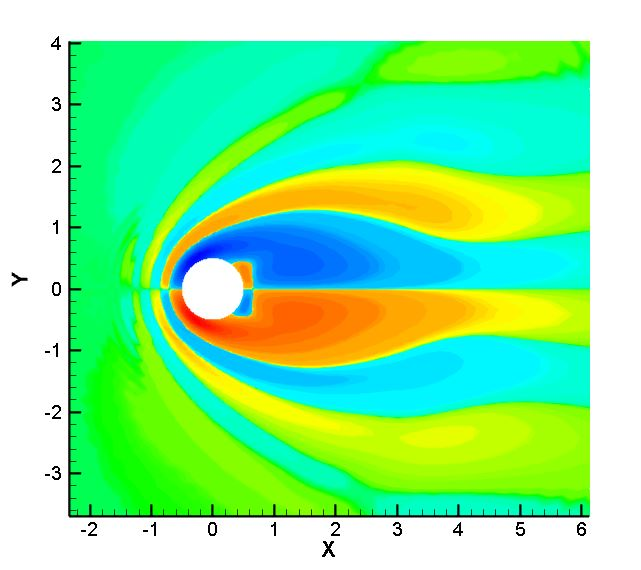
\includegraphics[height=7cm,width=7cm]{../pic/Vorticity_Contrast.JPG}
\caption{Re=200 \ 涡量云图}
\end{minipage}

\begin{minipage}{7cm}
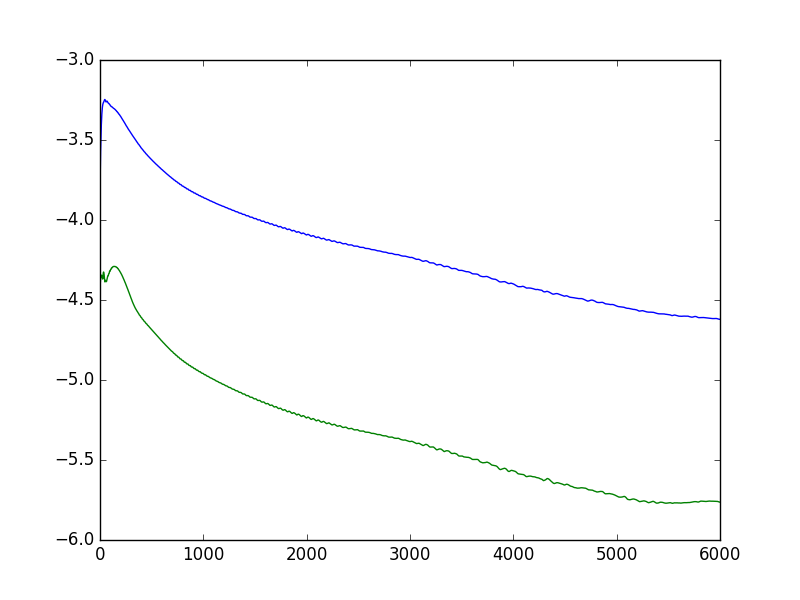
\includegraphics[height=7cm,width=7cm]{../pic/Residue_Contrast.png}
\caption{Re=200 \ 残差图}
\end{minipage}
\begin{minipage}{7cm}
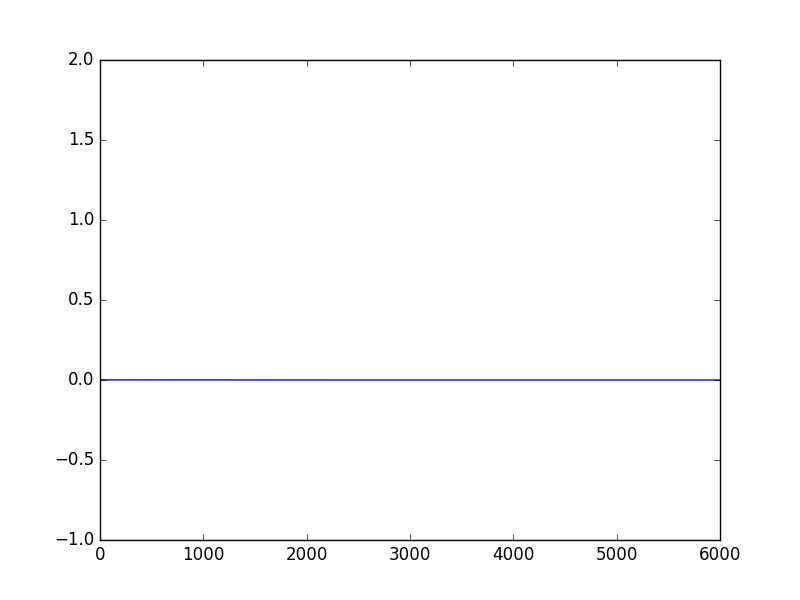
\includegraphics[height=7cm,width=7cm]{../pic/Aerodynamics_Contrast.png}
\caption{Re=200 \ 气动力系数}
\end{minipage}
\end{figure}\\
\indent 从上述4图可见,将网格变得粗糙些对最终结果影响不大,流场的特性仍然相同,但是残差的稳定性有细微变化,粗糙的网格使得残差更容易产生低频的波动。
\clearpage

\section{总结}
本文探究了使用TLLBM来模拟二维圆柱绕流的流场,编程实现了基于LBGK-D2Q9模型的TLLBM算法,使用贴体网格模拟了在Re=20,40,100,200这4种情况下的流场,数值仿真结果与实验数据吻合较好,表明TLLBM做为一种从介观角度发展而来的方法具有良好效果。\\
\indent 由于初次接触这种介观方法,本文对阻力系数的计算并未做深入研究,另外由于对LBM方法的理解还存在一些模糊的地方,还需要进一步探讨一些参数选择的原理。\\
\indent 虽然对于圆柱绕流而言贴体网格更为自然,但是正交的均匀或非均匀网格也可给出准确结果。由于时间关系,本文未做相应尝试。

\end{document}





































